\section{BP}
Ya conocemos el algoritmo de aprendizaje del gradiente descentente, y en esta sección veremos BP, que como ya hemos mencionado, es el algoritmo más usado a la hora de calcular el gradiente en el entrenamiento de un modelo. 

Cuando queremos obtener las predicciones de una red neuronal para unos datos de entrada concretos, la información fluye desde atrás hacia delante, es decir desde la capa de entrada $x$, pasando por las capas ocultas hasta producir una salida $o$, que si es evaluada con la función de coste $C$ produce un escalar $E$ que representa el error del modelo. A esto lo llamamos propagación hacia delante (\textit{forward propagation}).

Para calcular el gradiente de la función de coste respecto a los pesos del modelo necesitamos que la información fluya en sentido contrario, es decir, propagamos el error $E$, pasando por las capas ocultas, hasta la capa de entrada $x$. Esto se conoce como propagación hacia atrás (\textit{backpropagation}). El algoritmo de BP toma su nombre de aquí ya que durante su aplicación necesitamos que la información se propage hacia atrás. Si bien, no se trata del mismo concepto, ya que podemos propagar la información hacia detrás sin necesidad de calcular el gradiente, con lo que no estaremos usando BP.






\subsection{Diferenciación automática}

El algoritmo de BP se implementa en la práctica a través de la diferenciación automática \cite{AutomaticDiff}, que es un algoritmo más general para calcular derivadas y que engloba a BP. Se fundamenta en descomponer las funciones en una secuencia de operaciones fundamentales para calcular sus derivadas a través de la regla de la cadena, haciendo este cómputo muy eficiente. Por ello se distingue de la diferenciación simbólica, que manipula las expresiones matemáticas para encontrar derivadas, y de la diferenciación numérica, que calcula las derivadas a través de aproximaciones con diferencias finitas. Esta es la implementación que se usa en las librerías de aprendizaje automático más usadas, como TensorFlow 2 y PyTorch.

En la diferenciación automática existen dos estrategias para calcular un vector gradiente o una matriz jacobiana: diferenciación hacia delante y diferenciación hacia atrás. La diferencia reside  principalmente, en si realizamos multiplicaciones de un vector por un jacobiano (hacia atrás) o de un jacobiano por un vector (hacia delante). La elección dependerá de las dimensiones de la matriz jacobiana que queramos calcular, en otras palabras, debemos comparar la dimensión de la entrada y de la salida del modelo. Si la dimensión de entrada es mayor que la de salida, necesitaremos menos operaciones para calcular la matriz jacobiana si usamos la estrategia de diferenciación hacia atrás y viceversa. 

Debido a la estructura general de una red neuronal donde la dimensión de la entrada es mucho mayor que la de la salida, resulta más eficiente calcular el gradiente con la diferenciación hacia atrás, y esto es lo que entendemos como el algoritmo de BP: la información se propaga hacia atrás en el modelo mientras que se usa la diferenciación hacia atrás con el objetivo de calcular el gradiente del error del modelo con respecto a sus pesos. Si usáramos la diferenciación hacia delante, aunque estuviéramos propagando la información hacia atrás no estaríamos usando el algoritmo de BP, y además sería mucho más ineficiente la computación. Se suele decir de manera general que el algoritmo de BP es una aplicación concreta de la diferenciación automática hecho a medida para el entrenamiento de redes neuronales.


Vamos a explorar el algoritmo de BP de manera progresiva: en primer lugar veremos la diferenciación hacia delante y hacia atrás, viendo por qué es más eficiente usar la segunda y acotando este algoritmo general para llegar al algoritmo de BP, para lo que veremos como calcular la matriz Jacobiana de la salida de un perceptrón multicapa (MLP, por sus siglas en inglés) respecto a la entrada, en una situación que no será de entrenamiento, ya que no habrá parámetros entrenables, pero nos servirá para ilustrar el funcionamiento de BP. Luego veremos como obtenemos el gradiente del error con respecto a los pesos de cada capa usando el algoritmo de BP en un MLP con parámetros entrenables, concretando con ejemplos para las capas más comunmente utilizadas. Finalmente vamos a generalizar este concepto hacia modelos más abstractos usando grafos dirigidos acíclicos. 


Los MLP son un tipo de red neuronal, dividos en capas compuestas de nodos llamados neuronas, donde cada nodo de cada capa está conectado con todos los nodos de la capa siguiente. Son usados principalmente con datasets tabulares, es decir aquellos que sus datos vienen en formato de tabla. Usaremos esta arquitectura para realizar el desarrollo teórico ya que es más sencilla conceptualmente y la notación no resulta tan engorrosa. 

\subsection{Diferenciación hacia delante vs hacia atrás en un MLP}


Definimos nuestro modelo como $f: \mathbb{R}^n \rightarrow \mathbb{R}^m$, $o=f(x)$ con $x \in \mathbb{R}^n$  y $o \in \mathbb{R}^m$. Asumimos que $f$ es una composición de funciones:

$$f=f_k \circ f_{k-1} \circ \cdots \circ f_2 \circ f_1$$

Donde $k-1$ es el número de capas ocultas del MLP y $k+1$ el total de capas. Cada función $f_i$ representa el cálculo que se realiza en la capa $i$-ésima. Se tiene para $i \in \left \{ 1,...,k \right \}$


$$f_i: \mathbb{R}^{m_i} \rightarrow \mathbb{R}^{m_{i+1}}$$

$$f_i(x_i)=x_{i+1}$$

Donde la entrada del modelo viene representada en la primera capa, $x=x_1$. Además se tiene que $m_i=n, m_{k+1}=m, x_{k+1}=o$. Para obtener la predicción del modelo, $o=f(x)=f_k(x_k)$, necesitamos calcular el resultado de todas las capas intermedias $x_{i+1}=f_i(x_i)$. 

Podemos ver que la matriz jacobiana de la salida con respecto a la entrada $J_f(x) =  \mathbb{R}^{m\times n}$ puede ser calculada usando la regla de la cadena . Esto nos va a servir para ilustrar las diferencias entre la diferenciación hacia atrás y hacia delante


$$J_f(x) = \frac{\partial o}{\partial x} = \frac{\partial o}{\partial x_k} \frac{\partial x_k}{\partial x_{k-1}} \cdots \frac{\partial x_3}{\partial x_2} \frac{\partial x_2}{\partial x_1} =$$

$$\frac{\partial f_k(x_k)}{\partial x_k} \frac{\partial f_{k-1}(x_{k-1})}{\partial x_{k-1}} \cdots \frac{\partial f_2(x_2)}{\partial x_2} \frac{\partial f_1(x_1)}{\partial x_1}=$$

$$= J_{f_k}(x_k) J_{f_{k-1}}(x_{k-1}) \cdots J_{f_2}(x_2) J_{f_1}(x_1)$$

Se discute ahora como calcular el jacobiano $J_f(x)$ de manera eficiente. Recordamos que 

$$J_f(x_1)=\frac{\partial f(x_1)}{\partial x_1} =
\begin{pmatrix}
\frac{\partial f_1}{\partial x_1} & \cdots & \frac{\partial f_1}{\partial x_n} \\

\vdots & \ddots & \vdots \\
\frac{\partial f_m}{\partial x_1} & \cdots & \frac{\partial f_m}{\partial x_n} 
\end{pmatrix}
= 
\begin{pmatrix}
 \nabla f_1(x)^T\\
 \vdots \\
 \nabla f_m(x)^T \\
\end{pmatrix}=
\begin{pmatrix}
     \frac{\partial f}{\partial x_1} \cdots \frac{\partial f}{\partial x_n}
\end{pmatrix} \in \mathbb{R}^{m \times n}$$





Donde $\nabla f_i(x) ^T \in \mathbb{R}^{1 \times n} $ es la fila $i$-ésima de la matriz jacobiana y $\frac{\partial f}{\partial x_j} \in \mathbb{R}^m$ es la columna $j$-ésima, para $i=1,...,m$ y $j=1,...,n$.

Podemos extraer la fila $i$-ésima del jacobiano usando un producto vector-jacobiano (PVJ) de la forma $e_i^T J_f(x)$, donde $e_i \in \mathbb{R}^m$ es el vector de la base canónica. De manera análoga se puede extraer la columna $j$-ésima de $J_f(x)$ usando un producto jacobiano-vector (PJV) de la forma $J_f(x)e_j$, donde $e_j \in \mathbb{R}^n$. Se tiene entonces que el cálculo de la matriz jacobiana $J_f(x)$ equivale a $n$ PJV o $m$ PVJ. 


Para construir el jacobiano a partir de operaciones PJV o PVJ, podemos suponer que el cálculo del gradiente de $f_i(x)$ tiene el mismo coste computacional que el cálculo de la derivada parcial de f con respecto de alguna de las variables $x_j$. Por tanto la forma de cálculo de la matriz jacobiana que sea más eficiente depende de qué valor es mayor: si $n$ o $m$.



Si $n<m$ será más eficiente calcular $J_f(x)$ para cada columna $j\in \left \{1,...,n \right \}$ usando PJV de derecha a izquierda.

$$J_f(x)v=J_{f_k}(x_k) \cdots J_{f_2}(x_2) J_{f_1}(x_1) v$$

Donde $J_{f_k}(x_k)$ tiene tamaño $m \times m_{k-1}$, $J_{f_i}(x_i)$ tiene tamaño $m_i \times m_{i-1}$ para $i \in {2,...,k-1}$ y $J_{f_1}(x_1)$ tiene tamaño $m_1 \times n$ mientras que el vector columna $v$ será $n \times 1$. Esta multiplicación se puede calcular usando el agoritmo de diferenciación hacia delante, que es un tipo de algoritmo usado en diferenciación automática (ver algoritmo \ref{alg:fowdiff}). Asumiendo que $m=1, m_i=m_j$, el coste de computar $J_f(x)$ es $O(n^2)$.


Donde los elementos de la matriz fila $v_j, j \in \left \{1,...,n \right \}$ se corresponden con las derivadas parciales de la función del MLP respecto a la entrada de la capa $j$, es decir la columna $j$-ésima de la matriz jacobiana, $v_j=\frac{\partial f}{\partial x_j}$. 

Si $n>m$ es más eficiente calcular $J_f(x)$ para cada fila $i=1,...,m$ usando PVJ de izquierda a derecha. La multiplicación izquierda con un vector fila $u^T$ es 

$$u^TJ_f(x)=u^TJ_{f_k}(x_k) \cdots J_{f_2}(x_2) J_{f_1}(x_1)$$

Donde $u^T$ tiene tamaño $1 \times m$,  $J_{f_k}(x_k)$ tiene tamaño $m \times m_{k-1}$, $J_{f_i}(x_i)$ tiene tamaño $m_i \times m_{i-1}$ para $i \in {2,...,k-1}$ y $J_{f_1}(x_1)$ tiene tamaño $m_1 \times n$. Esto puede calcularse usando la diferenciación hacia atrás (ver algoritmo \ref{alg:backdif}). Asumiendo que $m=1, m_i=m_j$, el coste de computar $J_f(x)$ es $O(n^2)$.

 
\begin{algorithm}[H]
\caption{Diferenciación hacia delante}
\label{alg:fowdiff}
    \begin{algorithmic}
        \State $x_1 := x$
        \For{$j \in \left \{ 1,...,n\right \}$}
            \State $v_j := e_j \in \mathbb{R}^n$
        \EndFor
        \For{$i \in \left \{ 1,...,k \right \}$}
            \State $x_{i+1}:=f_i(x_i)$
            \For{$j \in \left \{ 1,...,n\right \}$}
                \State $v_j:= J_{f_i}(x_i)v_j$
            \EndFor
        \EndFor 

        
         \Return $o=x_{k+1}, \left (v_1, v_2, ..., v_n \right )$
        
    \end{algorithmic}
\end{algorithm}


\begin{algorithm}
\caption{Diferenciación en modo reverso}
\label{alg:backdif}
    \begin{algorithmic}
        \State $x_1:=x$
        \For{$k \in \left \{1,...,K \right \}$}
            \State $x_{k+1} = f_k(x_k)$
        \EndFor
        \For{$i \in \left \{1,...,m \right \}$}
            \State $u_i:=e_i \in \mathbb{R}^m$
        \EndFor 
        \For{$k \in \left \{ K,...,1 \right \}$}
            \For{$i \in \left \{ 1,...,m \right \}$}
                \State $u_i^T:= u_i^T J_{f_k}(x_k)$
            \EndFor
        \EndFor 

        \Return $o=x_{k+1}, \left ( u_1^T, u_2^T, ..., u_m^T \right )$
    \end{algorithmic}
\end{algorithm}

Donde los elementos $u_i^T$ se corresponden con el gradiente de la función $f_i$, $u_i^T=\nabla f_i(x)^T$, es decir la fila $i$-ésima de la matriz jacobiana. Este algoritmo aplicado al cálculo del gradiente del error del modelo con respecto a los pesos, propagando la información hacia atrás y con el objetivo de usar gradiente descendente, es lo que conocemos como BP.

Con la notación que estamos empleando, cuando $m=1$ el gradiente $\nabla f(x)$ tiene la misma dimensión que $x$. Por tanto es un vector columna mientras que $J_f(x)$ es un vector fila, por lo que técnicamente se tiene que $\nabla f(x)= J_f(x)^T$. Es de vital importancia aclarar esto ya que es el caso en el que nos situamos cuando usamos BP. La dimensión de salida siempre es uno, ya que calculamos la matriz jacobiana de la función de error del modelo con respecto a los pesos, con lo que será un vector gradiente de dimensión igual a la dimensión de los pesos del modelo. La predicción del modelo puede tener dimensión 1 en tareas de regresión, o una dimensión mayor que dos para tareas de clasificación, aunque de manera general no suele ser mayor de 100. La función de error del modelo siempre tendrá como imagen un valor escalar.


Acabamos de comprobar que para calcular una matriz jacobiana resulta más eficiente usando diferenciación hacia delante si la dimensión de la entrada es menor que la dimensión de la salida; y si la dimensión de la salida es menor que la dimensión de la entrada es preferible usar diferenciación hacia atrás. Por las características de las redes neuronales y los problemas en los que se aplican, siempre vamos a tener que la dimensión de salida es mucho menor que la dimensión de la entrada, por lo que es mucho más eficiente usar la diferenciación hacia atrás. 




\subsection{BP para MLP}


En la sección anterior hemos visto un modelo que no tenía ningún parámetro entrenable. Ahora usaremos uno que sí los tiene y veremos cómo calcular el gradiente de la función de coste con respecto a esos pesos. Los parámetros son valores reales y tienen la forma $W= W_1 \times W_2 \times \cdots \times W_k \subset \Omega$, y $W_i \in \mathbb{R}^{n_i \times n_{i+1}}$. $n_i$ es el número de neuronas de la $i$-ésima capa. El modelo que tendríamos añadiendo los pesos es $f: \mathbb{R}^n \times \Omega \rightarrow \mathbb{R}^m$, $o=f(x,W)$ con $x \in \mathbb{R}^n$  y $o \in \mathbb{R}^m$. Donde las funciones de cada capa son de la forma $f_i(x_i, W_i)= \sigma_i(W_ix_i)=x_{i+1}$ donde $\sigma_i$ es una función de activación generalmente no lineal. Dependiendo del tipo de problema, la función $f_k$ puede ser distinta: en un problema de regresión usamos la identidad, en clasificación usamos la función Softmax.


Ahora vamos a considerar la función de coste del modelo como una capa más, a parte de las funciones de las capas que nos permiten obtener la predicción. Siguiendo con la notación anterior, incluyendo la función de error $\mathcal{L}: \mathbb{R}^n \times \Omega \times \mathbb{R}^m \rightarrow \mathbb{R}$, $E=\mathcal{L}((x,W,y)= C(f(x,W),y)$, con $y \in \mathbb{R}^m$ siendo la etiqueta correcta para la entrada $x$ y $C: \mathbb{R}^m \times \mathbb{R}^m \rightarrow \mathbb{R}$ la función de coste del modelo. Con esto tenemos que $\mathcal{L} = C \circ f$. 

%TODO: revisar porque no he metido los bias a la hora de operar con los pesos del modelo.

\begin{ejemplo}
    Suponemos un MLP con dos capas ocultas, la salida escalar (problema de regresión) y una función de pérdida $C(f(x,W),y)=\frac{1}{2} \| f(x,W) - y\|^2$. Entonces tenemos $\mathcal{L}:\mathbb{R}^n \rightarrow \mathbb{R}$ y cada capa tiene equación

    
    
    \begin{gather*}
    f_1(x_1, W_1)=\sigma_1(W_1x_1)=x2 \\
      f_2(x_2, W_2)=W_2x_2=x_3=f(x,W)=o  \\
      C(f(x,W),y)= \frac{1}{2} \| x_3 - y \|^2 = E
    \end{gather*}

    


\end{ejemplo}

El objetivo, para poder aplicar el entrenamiento a través del gradiente descendente será calcular el gradiente del error con respecto a los parámetros $\frac{\partial E}{\partial W}$. Buscamos obtener un vector gradiente de la misma dimensión que $W$, pero el calculo no es directo, calcularemos progresivamente el gradiente de la función de coste con respecto a los pesos de cada capa, desde la capa final hasta la inicial por lo que buscamos calcular $\frac{\partial E}{\partial W_i}, \forall i=1,...,k$.  Para la última capa $\frac{\partial E}{\partial W_k}$ el cálculo es inmediato, mientras que para el resto podemos usar la regla de la cadena para obtener que 

$$\frac{\partial \mathcal{L}}{\partial W_i}=\frac{\partial \mathcal{L}}{\partial x_k} \frac{\partial x_k}{\partial x_{k-1}} \frac{\partial x_{k-1}}{\partial x_{k-2}} \cdots \frac{\partial x_{i+1}}{\partial W_i}$$

Cada $\frac{\partial \mathcal{L}}{\partial W_i}= \left ( \nabla_{W_i} \mathcal{L}^T \right )$ es un vector gradiente con el mismo número de elementos que $W_i$. Estos se calculan propagando hacia atrás la información en el modelo y usando la estrategia de diferenciación hacia atrás a través de PVJ, es decir, el algoritmo de BP que podemos ver en el pseudocódigo \ref{alg:BPMLPk}. 



\begin{algorithm}
\caption{BP para MLP con k capas}
\label{alg:BPMLPk}
    \begin{algorithmic}
        \State //Propagación hacia delante
        \State $x_1:=x$
        \For{$l \in \left \{1,...,L \right \}$}
            \State $x_{l+1}=f_k(x_l, W_l)$
        \EndFor

        \State //Propagación hacia atrás

        \State $u_{L+1}=1$
        \For{$l \in \left \{L,...,1 \right \}$}
            \State $g_l:= u_{l+1}^T \frac{\partial f_l(x_l, W_l)}{\partial W_l}$
            \State $u_l^T:=u_{l+1}^T\frac{\partial f_l(x_l, W_l)}{\partial x_l}$
        \EndFor
            

        \Return $\left \{  \nabla_{W_l}; l=1,...,L \right \}$
    \end{algorithmic}
\end{algorithm}


Para tener una idea más profunda y completa acerca del algoritmo de BP, vamos a ver como calcular el PVJ para las capas más comunes en los modelos, para lo que analizaremos sus matrices Jacobianas respecto de la entrada de la capa. 



\subsubsection{Capa no-lineal}



Consideramos primero una capa que aplica una función no lineal, normalmente el caso de las funciones de activación. $z=\sigma(x)$, con $z^(i) = \sigma(x^(i))$. El elemento en la posición $(i,j)$ del Jacobiano es dado por:

$$ \frac{\partial z^(i)}{\partial x^(j)} =  \left\{\begin{matrix}

\sigma'(x^(i)) \quad \textrm{si } i=j  \\
0 \quad \textrm{en otro caso}
\end{matrix}\right .
$$

Donde $\sigma'(a) = \frac{d}{da}\sigma(a)$. En otras palabras, el Jacobiano con respecto de la entrada es 

$$J=\frac{\partial \sigma}{\partial x}= diag(\sigma'(x))$$

Si tomamos como ejemplo la función ReLU, para un vector arbitratio $u$, podemos calcular su PVJ $u^TJ$ a través de la multiplicación  de elementos de la diagonal de $J$ con el vector $u$. 


$$\sigma(a) = ReLU(a)= max(a,0),$$
$$\sigma'(a)=
\left\{\begin{matrix}

0 \quad \textrm{si } a<0  \\
1 \quad \textrm{si } a>0
\end{matrix}\right.
$$

Como hemos visto en la sección \ref{sec:subgrad} la función ReLU no es diferenciable en el punto 0, pero sí que admite subderivada en todo su dominio, y en el punto $a=0$ es cualquier valor entre $[0,1]$, y usualmente en la práctica se toma el valor 0. Por tanto

$$ReLU'(a)= \left\{\begin{matrix}

0 \quad \textrm{si } a\leq0  \\
1 \quad \textrm{si } a>0
\end{matrix}\right.$$

$$J=\frac{\partial \sigma}{\partial x}= diag(ReLU'(x))$$


\subsubsection{Capa Cross Entropy}

Consideramos ahora la capa cuya función es la función de coste, en concreto con una medición del error usando Cross-Entropy Loss donde tenemos $C$ clases, que toma las predicciones $x$ y las etiquetas $y$ como entrada y devuelve un escalar. Recordamos que en esta capa la matriz Jacobiana es un vector fila, identificado con el gradiente, ya que la salida es un escalar.

$$z=f(x)=CrossEntropy(x,y)= - \sum_c y_c log(softmax(x)_c) = - \sum_c y_c log(p_c)$$

donde $p_c=softmax(x)_c= \frac{e^{x_c}}{\sum_{c'=1}^C e^{x_{c'}}}$ son las probabilidades de las clases predichas, e $y$ es la etiqueta correcta (codificado normalmente como un one-hot encoded vector). El Jacobiano con respecto a la entrada es

$$J= \frac{\partial z}{\partial x}= (p-y)^T \in \mathbb{R}^{1\times C}$$

Vamos a asumir que la clase objetivo es la etiqueta c:

$$z=f(x)=-log(p_c)=-log \left (\frac{e^{x_c}}{\sum_j e^{x_j}} \right ) = log \left ( \sum_j e^{x_j} \right ) - x_c$$

Entonces

$$\frac{\partial z}{\partial x_i} = \frac{\partial}{\partial x_i} log \sum_j e^{x_j} - \frac{\partial}{\partial x_i}x_c = \frac{e^{x_i}}{\sum_j e^{x_j}} - \frac{\partial}{\partial x_i}x_c = p_i - \mathbb{I}(i=c)$$

\subsubsection{Capa lineal}



Consideramos por último una capa lineal $z=f(x,W)=Wx$, donde $W \in \mathbb{R}^{m \times n}$, con $x \in \mathbb{R}^n$ y $z \in \mathbb{R}^m$ son respectivamente la entrada y la salida de esa capa.

Conviene aclarar, para evitar confusiones, que en la descripción previa hemos considerado las capas ocultas como una combinación de las operaciones lineales que aquí se describen con las funciones de activación, aquí sin embargo las analizamos por separado con el objetivo de una descripción má sencilla y un análisis más individualizado. Esta agrupación es una abstracción y por tanto no varía en cuanto a resultados.


Podemos calcular el Jacobiano de la función de la capa con respecto al vector entrada de esa capa, $J=\frac{\partial z}{\partial x} \in \mathbb{R}^{m \times n}$. Como

$$z_i = \sum_{l=1}^n W_{il}x_l$$

El elemento que ocupa la posición $(i,j)$ en la matriz Jacobiana será 

$$\frac{\partial z_i}{\partial x_j} = \frac{\partial}{\partial x_j} \sum_{l=1}^n W_{il} x_l = \sum_{l=1}^n W_{il} \frac{\partial}{\partial x_j} x_l = W_{ij}$$

ya que $\frac{\partial}{\partial x_j} x_l= \mathbb{I} (l=j)$. Por tanto el Jacobiano con respecto a la entrada será

$$J=\frac{\partial z}{\partial x}=W$$

El PVJ entre $u^T \in \mathbb{R}^{1 \times m}$ y $J \in \mathbb{R}^{m \times n}$ es

$$u^T \frac{\partial z}{\partial x} = u^T W \in \mathbb{R}^{1 \times n}$$

Ahora consideramos el Jacobiano con respecto a la matriz de los pesos, $J=\frac{\partial z}{\partial W}$. Esto se puede representar como una matriz de tamaño $m \times (m \times n)$, que resulta compleja de manejar. Por tanto en lugar de eso veremos de manera individual como calcular el gradiente con respecto a un único peso $W_{ij}$. Esto es más sencillo de calcular ya que $\frac{\partial z}{\partial W_{ij}}$ es un vector. Para su cómputo nos fijamos en que 

$$z_l = \sum_{t=1}^n W_{lt}x_t$$

$$\frac{\partial z_l}{\partial W_{ij}} = \sum_{t=1}^n x_t \frac{\partial}{\partial W_{ij}} W_{lt} = \sum_{t=1}^n x_t \mathbb{I}(i=l \textrm{ y } j=t) $$

Por tanto

$$\frac{\partial z}{\partial W_{ij}} = \left ( 0 \cdots 0 \quad x_j \quad 0 \cdots 0 \right )^T$$

Donde el elemento no nulo ocupa la posición $i$-ésima. El PVJ entre $u^T \in \mathbb{R}^{1 \times m}$ y $\frac{\partial z}{\partial W} \in \mathbb{R}^{m \times ( m \times n)}$ se puede representar como una matriz de tamaño $1 \times (m \times n)$. Vemos que 

$$u^T \frac{\partial z}{\partial W_{ij}}= \sum_{l=1}^m u_l \frac{\partial z_l}{\partial W_{ij}} = u_i x_j$$

Con lo cual

$$ u^T \frac{\partial z}{\partial W}  = ux^T \in \mathbb{R}^{m \times n}$$



\subsubsection{Grafos computacionales}

Los MLP son un tipo de Redes Neuronales Profundas donde cada capa se conecta directamente con la siguiente formando una estructura de cadena. Sin embargo las Redes Neuronales Profundas más recientes combinan componentes diferenciables de forma mucho más compleja, creando un grafo computacional de forma similar a como en la programación se combinan funciones simples para hacer otras más complejas. La restricción es que el grafo resultante debe de ser un Grafo Acíclico Dirigido, donde cada nodo es una función subdiferenciable. Vamos a ver un ejemplo usando la función $f(x_1,x_2)=x_2e^{x_1}\sqrt{x_1+x_2e^{x_1}}$, cuyo grafo se ver reflejado en la figura \ref{fig:def.grafo}.


\begin{figure}
    \centering
    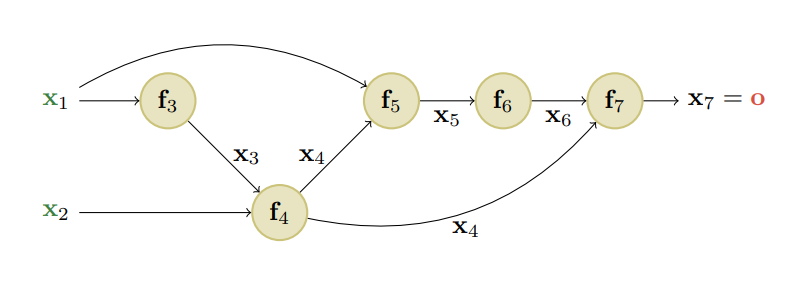
\includegraphics[width=1.0\linewidth]{Plantilla_TFG_latex/imagenes/Mat/Definicion/graf.png}
    \caption{Representación del grafodirigido acíclico (imagen obtenida de \ref{murphy2022probabilistic})}
    \label{fig:def.grafo}
\end{figure}


Las funciones intermedias que vemos en el grafo son:

\begin{gather*}
x_3= f_3(x_1)=e^{x_1} \\
x_4 = f_4(x_2,x_3)=x_2x_3 \\
x_5=f_5(x_1,x_4)=x_1 + x_4 \\
x_6=f_6(x_5) = \sqrt{x_5} \\
x_7=f_7(x_4,x_6)=x_4x_6 
\end{gather*}

Ahora no tenemos una estructura de cadena y puede que necesitemos sumar los gradientes a través de diferentes caminos, como es el caso del nodo $x_4$ que influye en $x_5$ y $x_7$. Para asegurar un funcionamiento correcto basta con nombrar los nodos en orden topológico (los padres antes que los hijos) y luego hacer la computación en orden topológico inverso. En general usamos

$$ \frac{\partial o }{ \partial x_j } = \sum_{k \in Hijos(j)} \frac{\partial o}{ \partial x_k} \frac{\partial x_k}{\partial x_j} $$

En nuestro ejemplo para el nodo $x_4$:

$$   \frac{\partial o }{ \partial x_4 }  =  \frac{\partial o}{ \partial x_5} \frac{\partial x_5}{\partial x_4} +\frac{\partial o}{ \partial x_7} \frac{\partial x_7}{\partial x_4} $$


En la práctica el grafo computacional se puede calcular previamente, usando una API que nos permita definir un grafo estático. Alternativamente podemos calcular el grafo en tiempo real, siguiendo la ejecución de la función en un elemento de entrada. Esta segunda opción hace más fácil trabajar con grafos dinámicos cuya forma pueden cambiar dependiendo de los valores calculados por la función. Por ejemplo, Tensorflow 1 usaba los grafos estáticos mientras que su versión más reciente TensorFlow 2 y PyTorch usan los grafos en tiempo real. 




\subsection{Problemas con el cálculo del gradiente}

\subsubsection{Desvanecimiento y explosión del gradiente}


Siguiendo el hilo de la sección \ref{sec:convergencia}, vamos a ver dos problemas que surgen a la hora de entrenar modelos usando gradiente descendente y que lastran la convergencia, pero con la diferencia de que estos están ligados únicamente al algoritmo de BP, es decir, a cómo se calcula el gradiente y no a cómo se usa en la búsqueda de soluciones.

Cuando entrenamos modelos muy profundos (con muchas capas ocultas), los gradientes tienen tendencia bien a volverse muy pequeños (desvanecimiento del gradiente) o bien a volverse muy grandes (explosión del gradiente) ya que el señal de error es pasada a través de una serie de capas que o lo amplifican o lo mitigan. Esto provoca que o bien se deje de actualizar el peso que se desvanece su gradiente o que el gradiente diverja en el otro caso \cite{VanishExplode}. Para ver el problema con detalle, consideramos el gradiente de la función de pérdida con respecto a un nodo en la capa $l$:

$$\frac{\partial \mathcal{L}}{\partial z_l} = \frac{\partial \mathcal{L}}{\partial z_{l+1}} \frac{\partial z_{l+1}}{\partial z_l} = g_{l+1} J_l$$

donde $J_l = \frac{\partial z_{l+1}}{\partial z_l}$ es la matriz jacobiana, y $g_{l+1} = \frac{\partial \mathcal{L}}{\partial z_{l+1}}$ es el gradiente de la siguiente capa. Si $J_l$ es constante entre capas, es claro que la contribución del gradiente de la capa final $g_L$ a la capa $l$ será $ g_L J^{L-l}$. Entonces el comportamiento del sistema dependerá de los valores propios de $J$. %TODO: Referencia o explicacion??

$J$ es una matriz de valores reales pero generalmente no es simétrica, por lo que sus autovalores y autovectores pueden ser complejos, representando un comportamiento oscilatorio. Sea $\lambda$ el radio espectral de $J$, que es el máximo del valor absoluto de sus autovalores. Si es mayor que 1, el gradiente puede explotar; y si es menor que 1 su gradiente se puede desvanecer. 

El problema de la explosión del gradiente se puede resolver de manera rápida y cómoda a través de acotar el gradiente con su magnitud y una constante $c \in \mathbb{R}^+$ en caso de que se vuelva muy grande.

$$g' = min(1, \frac{c}{\|g\|}g)$$

De esta manera la norma de $g'$ nunca puede ser mayor que c, pero el vector apunta siempre en la misma dirección que el gradiente.

También existen otras soluciones que además son aplicables al problema del desvanecimiento de gradiente, que no se soluciona de manera tan sencilla:

\begin{itemize}
    \item Adaptar las funciones de activación para prevenir que el gradiente se vuelva muy grande o muy pequeño.

    \item Modificar la arquitectura para estandarizar las funciones de activación en cada capa, para que la distribución de las activaciones sobre el conjunto de datos permanezca constante durante el entrenamiento.

    \item Elegir cuidadosamente los valores iniciales de los pesos del modelo.
   
\end{itemize}

En la siguiente sección veremos detenidamente el último punto, ya que es la práctica más estandarizada. 


\subsubsection{Inicialización de los pesos}

La manera en la que inicializamos los pesos es una decisión importante a la hora de determinar cómo converge (y si lo hace) un modelo. La convergencia o no, su velocidad y la solución a la que se converge en el entrenamiento de un modelo mediante el algoritmo de gradiente descendente es muy sensible al punto inicial desde el que comenzamos la búsqueda de una solución. Hay que remarcar que esto sucede cuando la función de error no es convexa, pero como es el caso mayoritario, lo asumimos de manera general.  

Basándonos en \cite{stabilityProblem2}, donde se observa que muestrear parámetros de una distribución normal con varianza fija puede resultar en el problema de la explosión de gradiente, vamos a ver por qué ocurre esto y, a través de añadir restricciones para evitarlo vamos a llegar a las heurísticas de inicialización de pesos más comunes.

Consideramos el pase hacia delante en una neurona lineal sin capa de activación dada por $o_i = \sum_{j=1}^{n_{in}} w_{ij}x_j$ . Suponemos $w_{ij} \sim \mathcal{N}(0, \sigma^2)$, y $\mathbb{E}[x_j]=0$ y $\mathbb{V}[x_j]=\gamma^2$, donde asumimos $x_j$ independiente de $w_{ij}$, y $n_{in}$ es el número de conexiones de entrada que recibe la neurona. La media y la varianza de la salida vienen dadas por

$$\mathbb{E}[o_i]= \sum_{j=1}^{n_{in}} \mathbb{E}[w_{ij} x_j] = \sum_{j=1}^{n_{in}} \mathbb{E}[w_{ij}] \mathbb{E}[x_j]=0$$

$$\mathbb{V}[o_i] = \mathbb{E}[o_i^2] - (\mathbb{E}[o_i])^2 = \sum_{j=1}^{n_{in}} \mathbb{E}[w_{ij}^2x_j^2] - 0 = \sum_{j=1}^{n_{in}} \mathbb{E}[w_{ij}^2] \mathbb{E}[x_j^2] = n_{in} \sigma^2 \gamma^2$$

Para evitar que la varianza diverja, necesitamos que $n_{in} \sigma^2$ se mantenga constante. Si consideramos el pase hacia atrás y realizamos un razonamiento análogo vemos que la varianza del gradiente puede explotar a menos que $n_{out} \sigma^2$ sea constante, donde $n_{out}$ son las conexiones de salida de la neurona. Para cumplir con esos dos requisitos, imponemos $\frac{1}{2}(n_{in}+n_{out}) \sigma^2 = 1$, o equivalentemente

$$\sigma^2= \frac{2}{n_{in}+n_{out}}$$

Esta se conoce como inicialización de Xavier o inicialización de Glorot \cite{stabilityProblem2}. Si usamos $\sigma^2= \frac{1}{n_{in}}$ tenemos un caso especial conocida como la inicialización de LeCun, propuesta por Yann LeCun en 1990. Es equivalente a la inicialización de Glorot cuando $n_{in}=n_{out}$. Si usamos $\sigma^2 = \frac{2}{n_{in}}$, tenemos la llamada inicialización de He, propuesta por Kaiming He en \cite{heinic}.


Cabe resaltar que no ha sido necesario usar una distribución Gaussiana. De hecho, las derivaciones de arriba funcionan en términos de la media y la varianza, y no hemos hecho suposiciones sobre si era Gaussiana. 


Aunque hemos supuesto que se trataba de una neurona lineal sin función de activación que añada una componente no lineal, se conoce de manera empírica que estas técnicas son extensibles a unidades no lineales. La inicialización que usemos dependerá mayoritariamente de la función de activación que usemos. Se conoce que para funciones de activación ReLU funciona mejor la inicialización de He, para las funciones SELU se recomienda la inicialización de LeCun y para las funciones lineales, logística, tangente hiperbólica y softmax se recomienda el uso de la inicialización de Glorot \cite{murphy2022probabilistic}.